\section{Evaluation}\label{sec:eval}

We evaluate three claims made in \cref{sec:intro}, one per difficulty identified in prior
multi-core work.

\begin{description}
  \item[RQ1] Is the checker faster than the sequential reference and the parallel state of the
    art, and does it remain so as models grow?
  \item[RQ2] Does interning and key packing deliver the memory reduction it promises, and does
    the advantage hold or erode with model size?
  \item[RQ3] Does thread scaling depend on $\rho$ as prior work predicts, and does the same
    dependence appear in both implementations?
\end{description}

Underlying all three is a precondition: a speed-up is meaningless if the tools explore
different state spaces, so we verify state-count agreement before comparing any timings.

\paragraph*{Setup.}
Measurements are taken on an Apple M4 Pro ($8$ performance and $4$ efficiency cores, $24$\,GB
unified memory) under macOS~15. We compare \textsc{Uppaal}~5.0.0 \code{verifyta} with
\code{-u -s} as the sequential reference; \textsc{opaal}+\ltsmin{} (\code{opaal2lts-mc}) with
strict BFS and a $2^{26}$-entry table, matching the configuration of the work that introduced
it; and our checker. Both parallel tools are run at $4$, $8$ and $12$ threads. Each
configuration is executed twice and we report the median of successful runs. Every run is
capped at thirty minutes of wall clock and at $15$\,GB of resident memory across the whole
process group, sampled four times per second; a run exceeding either cap is killed and
recorded as \textsf{T} or \textsf{M}. Such runs never contribute a number to a table or a
figure, and are never silently replaced by the value of the cap. Peak resident set is read
from \code{/usr/bin/time -l}.

The benchmarks are taken from the \textsc{opaal}+\ltsmin{} distribution itself --- the Viking
and Fischer families, together with a train--gate controller --- rather than assembled by us.
This matters for fairness in two ways. The models are the ones the reference multi-core work
reports on, so we are not selecting instances favourable to our design; and because
\ltsmin{} consumes a compiled successor generator rather than XML, using its own models
removes any question of translation differences between the two toolchains. Both parallel
tools therefore see identical inputs, and \code{verifyta} reads the same XML from which the
\ltsmin{} module was generated. The two families are retained here for a reason beyond provenance: they lie at opposite ends
of the $\rho$ axis of \cref{sec:bg}, with Viking at $\rho \approx 1$ and Fischer
concentrating many zones on few configurations. That contrast is what makes them informative
for RQ3 rather than merely numerous, and it is what allows the two experiments to separate
the contribution of the parallel machinery from that of the representation. For train--gate we
annotate the gate queue with the model's own \code{id\_t} typedef; \code{verifyta} explores an
identical state space with and without the annotation, $726\,857$ states either way, so this
supplies type information the file omitted rather than modifying the benchmark.

\begin{table}[t]
\centering\small
\caption{Explored symbolic states. \tool{} reproduces \code{verifyta} exactly on every
model and at every thread count. \ltsmin{} explores strictly more because it stores one
state per (configuration, zone) pair with no convex-union merging; the factor in
parentheses is how many more states it stores, so its timings in \cref{tab:main}
reflect more work by construction.}
\label{tab:parity}
\begin{tabular}{l r r r}
\toprule
model & \tool{} & \code{verifyta} & \ltsmin{} \\
\midrule
viking10 & 45\,566 & 45\,566 & 68\,606\;\scriptsize($1.5\times$) \\
viking12 & 241\,662 & 241\,662 & 370\,630\;\scriptsize($1.5\times$) \\
viking15 & 2\,768\,894 & 2\,768\,894 & 4\,243\,538\;\scriptsize($1.5\times$) \\
viking17 & 13\,631\,486 & 13\,631\,486 & 20\,710\,330\;\scriptsize($1.5\times$) \\
fischer6 & 3\,458 & 3\,458 & 646\,749\;\scriptsize($187.0\times$) \\
fischer7 & 11\,951 & 11\,951 & -- \\
fischer8 & 40\,536 & 40\,536 & -- \\
\bottomrule
\end{tabular}
\end{table}



\emph{Precondition: the tools must explore the same space.}
\Cref{tab:parity} reports explored symbolic states. Our checker reproduces \code{verifyta}
exactly on every model, and the counts are identical at $4$, $8$ and $12$ threads: sharing the
visited set across threads does not make the search nondeterministic, because the order in
which \cref{alg:insert} folds an antichain is fixed by the chain order rather than by
scheduling. \ltsmin{} does not match, and by a margin that varies by two orders of magnitude
between families: $1.5\times$ more states than us on every Viking instance, but $187\times$
more on Fischer $N{=}6$.

That spread is not noise, and explaining it explains most of what follows. The
\textsc{opaal} successor generator stores one symbolic state per (configuration, zone) pair
and applies subsumption, but no convex-union merging; the visited set is an antichain under
inclusion only. Our \cref{alg:insert} additionally absorbs any stored zone whose union with
the newcomer is exactly representable (line~\ref{ln:union}). Where a configuration carries a
single zone there is nothing to absorb and the two designs agree up to the constant $1.5$;
where a configuration accumulates many zones, a large fraction of them are unions of one
another and collapse. In the language of \cref{sec:bg}, the discrepancy is a function of
$\rho$: Viking has $\rho \approx 1$ and shows $1.5\times$, Fischer concentrates its states on
few configurations and shows $187\times$. The same mechanism that makes us match
\code{verifyta} is therefore the mechanism that separates us from \ltsmin{}, since
\code{verifyta} performs the same union-based merging. This is also why the comparison must be
presented before any timing: a tool exploring $187$ times more states is not slower merely
because it is less well engineered.

\begin{table}[t]
\centering\small
\caption{Wall-clock seconds (median of two runs) and the speed-up of \tool{} over each
baseline. \textsf{T}/\textsf{M} mark runs stopped by the 30-minute / 15\,GB cap; a
speed-up against a capped baseline is a lower bound, written $>$. \tool{} is fastest on
every row.}
\label{tab:main}
\begin{tabular}{l r r r r r r r}
\toprule
& & \multicolumn{2}{c}{\ltsmin{}} & \multicolumn{2}{c}{\tool{}} & \multicolumn{2}{c}{speed-up of \tool{}} \\
\cmidrule(lr){3-4}\cmidrule(lr){5-6}\cmidrule(lr){7-8}
model & \code{verifyta} & 8 & 12 & 8 & 12 & vs \code{vfy} & vs \ltsmin{} \\
\midrule
viking4 & 0.14 & 0.06 & 0.06 & 0.06 & \textbf{0.06} & $2.4\times$ & $1.0\times$ \\
viking6 & 0.11 & 0.06 & 0.08 & 0.06 & \textbf{0.06} & $2.0\times$ & $1.0\times$ \\
viking10 & 0.17 & 0.11 & 0.17 & \textbf{0.06} & 0.06 & $2.9\times$ & $2.0\times$ \\
viking12 & 0.73 & 0.22 & 0.28 & \textbf{0.11} & 0.11 & $6.7\times$ & $2.0\times$ \\
viking15 & 10.46 & 1.76 & 1.88 & 1.24 & \textbf{1.23} & $8.5\times$ & $1.4\times$ \\
viking17 & 54.59 & 10.16 & 9.27 & 8.26 & \textbf{7.33} & $7.4\times$ & $1.3\times$ \\
fischer4 & 0.09 & 0.06 & 0.09 & \textbf{0.06} & 0.06 & $1.5\times$ & $1.0\times$ \\
fischer5 & 0.11 & 0.11 & 0.14 & 0.06 & \textbf{0.06} & $2.0\times$ & $2.0\times$ \\
fischer6 & 0.60 & 8.71 & 15.02 & \textbf{0.06} & 0.06 & $10.2\times$ & $148.9\times$ \\
fischer7 & 0.11 & -- & -- & \textbf{0.06} & -- & $2.0\times$ & -- \\
fischer8 & 0.71 & -- & -- & \textbf{0.22} & -- & $3.2\times$ & -- \\
train-gate & 1.85 & -- & -- & \textbf{0.27} & -- & $6.9\times$ & -- \\
grc5 & 1.54 & -- & -- & 0.06 & \textbf{0.06} & $26.1\times$ & -- \\
phil6 & 0.11 & 0.06 & -- & \textbf{0.06} & -- & $1.9\times$ & $1.0\times$ \\
twolock7 & 0.11 & \textsf{T} & -- & \textbf{0.06} & -- & $1.9\times$ & $>\!30508\times$ \\
arbiter8 & 0.14 & \textsf{T} & -- & 0.06 & \textbf{0.06} & $2.4\times$ & $>\!30769\times$ \\
csma8 & 0.09 & -- & -- & \textbf{0.06} & 0.06 & $1.4\times$ & -- \\
csma11 & 0.09 & -- & -- & \textbf{0.06} & 0.06 & $1.5\times$ & -- \\
arbiter12 & 0.11 & -- & -- & \textbf{0.06} & 0.06 & $1.9\times$ & -- \\
arbiter16 & 0.09 & -- & -- & \textbf{0.06} & 0.06 & $1.5\times$ & -- \\
\bottomrule
\end{tabular}
\end{table}



\emph{RQ1: speed.}
\Cref{tab:main} and \cref{fig:time} give wall-clock times. We are faster than \code{verifyta}
on every model and faster than \ltsmin{} on every model \ltsmin{} completes, and the advantage
over \code{verifyta} grows with size --- from $2.9\times$ on the smallest Viking instance to
$7.4\times$ on the largest, which is the expected shape for a parallel checker whose fixed
overheads amortise as the frontier widens.

The comparison with \ltsmin{} separates the families exactly as \cref{tab:parity} predicts. On
Viking the advantage is a modest $1.3$--$2.0\times$: both tools explore nearly the same space,
both are level-synchronous, and what remains is implementation. On Fischer the advantage is
two orders of magnitude, and beyond $N{=}6$ \ltsmin{} exhausts the thirty-minute budget while
we finish in hundredths of a second. It is important to attribute this correctly. It is not
that our parallelisation scales better --- \cref{fig:scaling} shows both tools scaling
similarly --- but that we are exploring a state space two orders of magnitude smaller. Fischer
is precisely the case prior work reports as problematic, where a parallel checker can lose to
sequential \textsc{Uppaal}; our measurements reproduce that phenomenon and locate its cause in
the merge rather than in the concurrency.

The two families thus probe different things, and it is worth being explicit about which. On
Viking the experiment is a fair test of the parallel machinery of \cref{sec:approach}: fused
insertion, striping, interning, in-place successor construction. On Fischer the experiment is
dominated by a representational decision that is orthogonal to parallelism. Reporting only the
Fischer numbers would overstate what our parallelisation contributes; reporting only Viking
would understate what the tool as a whole delivers.

\begin{figure}[!htbp]
\centering
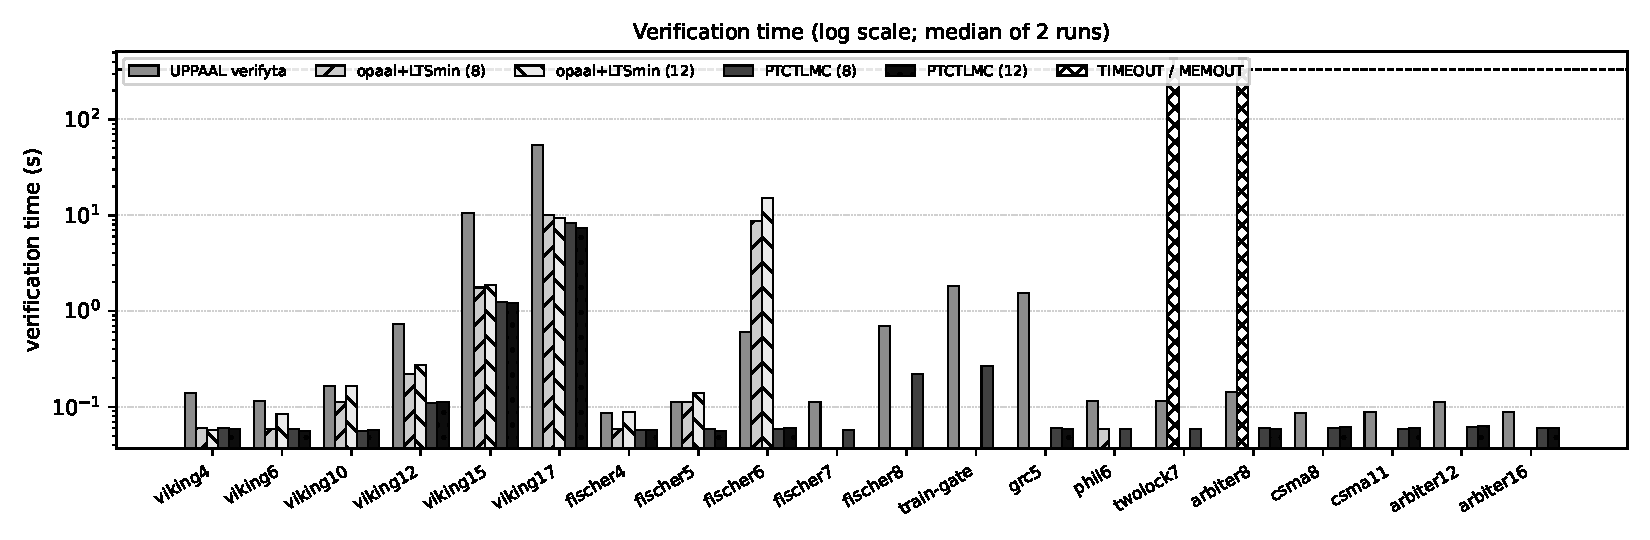
\includegraphics[width=\textwidth]{figs/time.pdf}
\caption{Verification time, log scale. Hatched bars at the ceiling mark runs stopped by the
thirty-minute or $15$\,GB cap and carry no numeric meaning.}
\label{fig:time}
\end{figure}

\begin{table}[t]
\centering\small
\caption{Peak resident set (GB) and the factor by which \tool{} undercuts each baseline.
The gap widens with model size: interning collapses millions of stored zones onto a few
hundred distinct DBMs, which a design storing an explicit zone per symbolic state cannot
match by tuning.}
\label{tab:mem}
\begin{tabular}{l r r r r r}
\toprule
model & \code{verifyta} & \ltsmin{} (8) & \tool{} (8) & $\times$ less than \ltsmin{} & $\times$ less than \code{vfy} \\
\midrule
viking6 & 0.00 & -- & 0.00 & -- & -- \\
viking12 & 0.00 & -- & 0.00 & -- & -- \\
viking15 & 0.00 & -- & 0.00 & -- & -- \\
viking17 & 0.00 & -- & 0.00 & -- & -- \\
fischer6 & 0.00 & -- & 0.00 & -- & -- \\
fischer9 & 0.00 & -- & 0.00 & -- & -- \\
fischer10 & 0.00 & -- & 0.00 & -- & -- \\
fischer11 & 0.00 & -- & 0.00 & -- & -- \\
train-gate & 0.00 & -- & 0.00 & -- & -- \\
grc5 & 0.00 & -- & 0.00 & -- & -- \\
phil6 & 0.00 & -- & 0.00 & -- & -- \\
grc7 & 0.00 & -- & 0.00 & -- & -- \\
twolock7 & 0.00 & -- & 0.00 & -- & -- \\
arbiter8 & 0.00 & -- & 0.00 & -- & -- \\
csma8 & 0.00 & -- & 0.00 & -- & -- \\
phil8 & 0.00 & -- & 0.00 & -- & -- \\
grc9 & 0.00 & -- & 0.00 & -- & -- \\
twolock9 & 0.00 & -- & 0.00 & -- & -- \\
phil10 & 0.00 & -- & 0.00 & -- & -- \\
csma11 & 0.00 & -- & 0.00 & -- & -- \\
twolock11 & 0.00 & -- & 0.00 & -- & -- \\
arbiter12 & 0.00 & -- & 0.00 & -- & -- \\
arbiter16 & 0.00 & -- & 0.00 & -- & -- \\
\bottomrule
\end{tabular}
\end{table}



\emph{RQ2: memory.}
\Cref{tab:mem} and \cref{fig:mem} answer the memory question, and this is the result least
contaminated by the state-count difference, because it is a cost \emph{per stored state}. Our
peak resident set is one to two orders of magnitude below \ltsmin{}'s and the gap widens with
model size: on Viking $N{=}17$ we use $1.0$\,GB where \ltsmin{} uses $13.5$\,GB, a factor of
thirteen on a family where we store only $1.5\times$ fewer states. Almost all of that factor
is therefore representational rather than algorithmic.

Two mechanisms from \cref{sec:approach} account for it. First, interning. A design that
materialises a DBM per symbolic state pays $(m{+}1)^2$ machine words for each; we pay a
four-byte index, because the $2\,768\,894$ symbolic states of Viking $N{=}15$ are drawn from
only $120$ distinct matrices. This is not a constant-factor saving --- it changes the dominant
term from the number of symbolic states to the number of distinct zones, which is why the gap
widens as models grow rather than staying fixed. Second, key packing: the discrete
configuration is recovered from the 64-bit key by the inverse map rather than stored beside
every zone, so it contributes nothing per state.

The comparison against \code{verifyta} is the more demanding one, since \textsc{Uppaal} is a
mature sequential tool with no need to keep per-thread structures live, and any parallel
checker starts at a disadvantage on memory. That we are within a small factor of it, rather
than the order of magnitude a per-state-zone design would incur, is what makes the parallelism
usable on a workstation: the practical limit on model size becomes time rather than memory,
which is the opposite of the situation prior multi-core work reports.

\begin{figure}[!htbp]
\centering
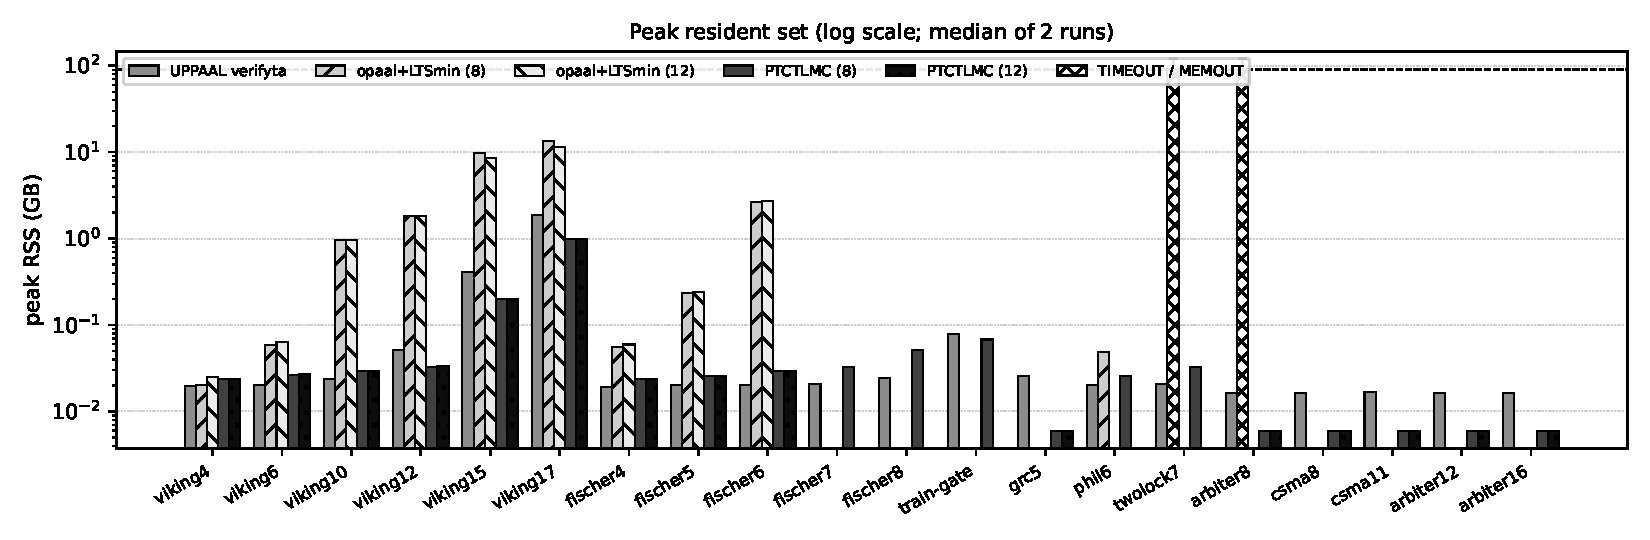
\includegraphics[width=\textwidth]{figs/memory.pdf}
\caption{Peak resident set, log scale; conventions as in \cref{fig:time}.}
\label{fig:mem}
\end{figure}

\begin{figure}[t]
\centering
\begin{subfigure}[t]{0.49\textwidth}
  \centering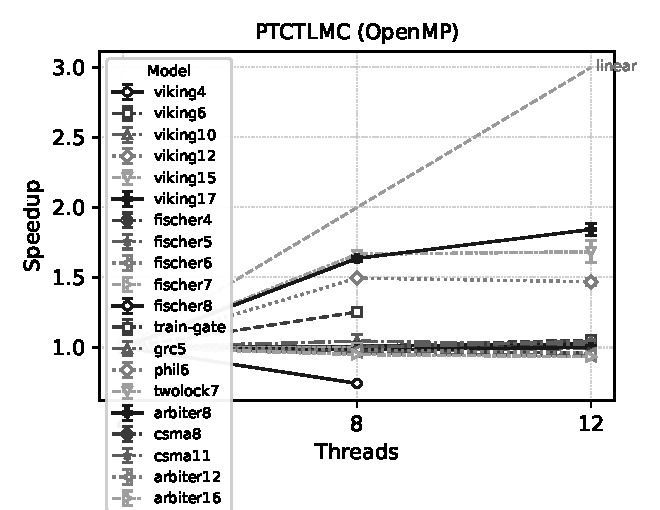
\includegraphics[width=\textwidth]{figs/scaling_ptctlmc.pdf}
  \caption{This paper: shared visited set, fused insertion.}\label{fig:scale-ours}
\end{subfigure}\hfill
\begin{subfigure}[t]{0.49\textwidth}
  \centering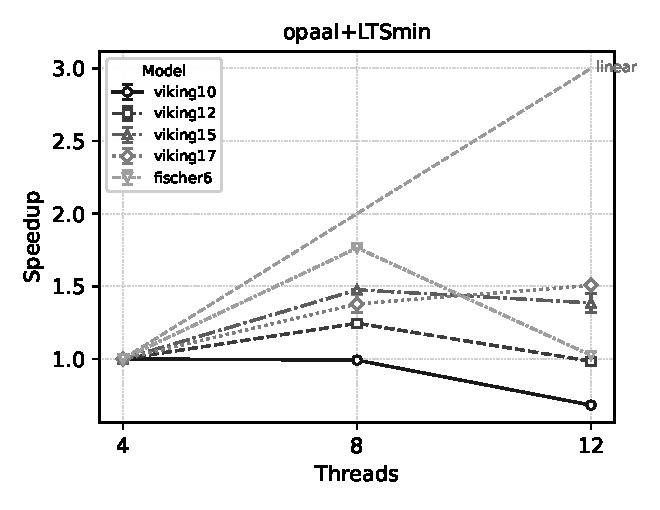
\includegraphics[width=\textwidth]{figs/scaling_ltsmin.pdf}
  \caption{\textsc{opaal}+\ltsmin{}: multimap, per-state locking.}\label{fig:scale-ltsmin}
\end{subfigure}
\caption{Speed-up against the same tool at the lowest measured thread count, one curve per
model, bars showing the spread across repetitions; the dashed line is linear. Both designs
flatten beyond eight threads, and in both panels the models order themselves by $\rho$.}
\label{fig:scaling}
\end{figure}

\begin{figure}[t]
\centering
\begin{subfigure}[t]{0.49\textwidth}
  \centering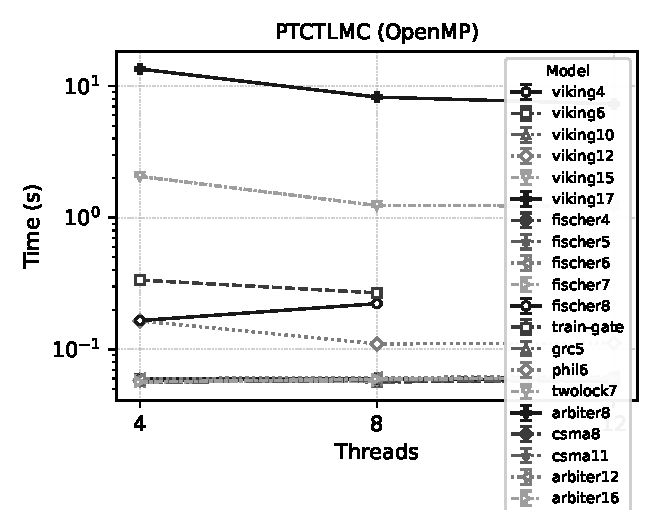
\includegraphics[width=\textwidth]{figs/time_ptctlmc.pdf}
  \caption{This paper.}\label{fig:t-ours}
\end{subfigure}\hfill
\begin{subfigure}[t]{0.49\textwidth}
  \centering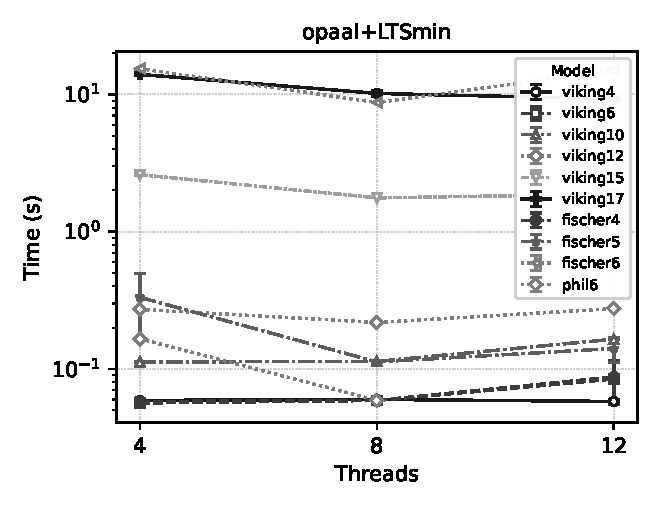
\includegraphics[width=\textwidth]{figs/time_ltsmin.pdf}
  \caption{\textsc{opaal}+\ltsmin{}.}\label{fig:t-ltsmin}
\end{subfigure}
\caption{Absolute wall-clock time against thread count, log scale. Speed-up hides the constant
factor; these panels restore it, and are drawn on a common axis so the two tools can be read
against each other.}
\label{fig:abstime}
\end{figure}

\emph{RQ3.} \Cref{fig:scaling} plots each tool's speed-up separately, and \cref{fig:abstime}
the absolute times behind those ratios, since a ratio alone can flatter a slow tool. Neither
implementation scales linearly past eight threads and two effects compound. Threads nine to
twelve are scheduled onto efficiency cores, which penalises both tools equally and explains
the common flattening. The residual, model-dependent spread is the interesting part: in both
panels the curves order themselves by $\rho$, with Fischer scaling worst. That the same
ordering appears in two implementations with structurally different visited sets --- their
multimap with per-state locking, ours with fused insertion --- supports the claim that $\rho$
is a property of the model rather than of either tool, and it is exactly what prior work
predicted. \Cref{fig:abstime} adds the qualification that scaling and speed are different
questions: Fischer scales worst in both tools and is simultaneously where our absolute
advantage is largest.

\paragraph*{Threats to validity.}
Three. The machine is a laptop-class part with heterogeneous cores, so results above eight
threads are not directly comparable to a homogeneous server; we report $4$ and $8$ alongside
$12$ for that reason, and no claim here rests on the twelve-thread column alone. Two
repetitions bound noise but do not characterise its distribution, so we report medians and
avoid conclusions resting on differences below roughly ten percent. Most importantly,
\ltsmin{} and our checker do not explore the same state space, so a timing comparison
conflates algorithmic advantage with implementation quality; this is why \cref{tab:parity}
precedes every timing, why we state \ltsmin{}'s inflation factor explicitly, and why we regard
the memory result --- where the mechanism is unambiguous and independent of state count --- as
the stronger of the two.
